\documentclass[10pt]{article}
\usepackage{amsmath}
\usepackage{graphicx}
\usepackage{geometry}
\usepackage{fancyhdr} % For header and footer
\usepackage{enumitem} % For customizing enumerate
\usepackage{tikz}
\usepackage{caption}
\usepackage{pgfplots}
\usetikzlibrary{3d,calc}
\geometry{letterpaper, margin=0.75in}
\renewcommand{\familydefault}{\sfdefault} % Use a sans-serif font

% Header and Footer
\pagestyle{fancy}
\fancyhf{}
\fancyhead[L]{EMCH 371 - Homework 3}
\fancyhead[R]{J. Vaught}
\fancyfoot[C]{\thepage}

% Title formatting
\title{\vspace{-2cm}\hrule\vspace{0.5cm}\\EMCH 371 - Homework 3 \vspace{0.5cm}\hrule}
\author{\vspace{-1cm}J. Vaught}
\date{\vspace{-0.2cm}Due: Tuesday, 10/22/2024}

\begin{document}
\maketitle

\vspace{-0.4cm}
\hrule
\vspace{0.5cm}

\section*{Problem 1}

\noindent \textbf{(Total 20 points)} Consider the 1040 carbon steel that has a Young's modulus of 200 GPa, and a Yield Strength (Y.S.) of 600 MPa.

\begin{enumerate}
    \item[(a)] A 20-mm diameter rod of this alloy is used as a structural member in an engineering design. The unstressed length of the rod is precisely \(1 \, \text{m}\). The structural load on the rod is \(9 \times 10^4 \, \text{N}\) in tension. What will be the length of the rod under this structural load? (10 points)

    \begin{align*}
        A &= \frac{\pi D^2}{4} = \frac{\pi (0.02 \, \text{m})^2}{4} = 3.14 \times 10^{-4} \, \text{m}^2
    \end{align*}

    \begin{align*}
        \Delta L &= \frac{P L_0}{A E} = \frac{9 \times 10^4 \, \text{N} \times 1 \, \text{m}}{(3.14 \times 10^{-4} \, \text{m}^2) \times (200 \times 10^9 \, \text{Pa})} \\
        &= 0.0014 \, \text{m}
    \end{align*}
\noindent
    Therefore, the new length of the rod under this load is:
    \begin{align*}
        L = 1.0014 \, \text{m}
    \end{align*}

    \item[(b)] A design engineer is considering a structural change that will increase the tensile load on this member. What is the maximum tensile load that can be permitted without producing extensive plastic deformation of the rod? (10 points)

    \begin{align*}
        P_{\text{max}} &= \text{Y.S.} \times A = (600 \times 10^6 \, \text{Pa}) \times (3.14 \times 10^{-4} \, \text{m}^2) \\
        &= 188,496 \, \text{N}
    \end{align*}
\end{enumerate}

\section*{Problem 2}

\noindent \textbf{(Total 10 points)}If the modulus of elasticity in the body-centered-cubic (BCC) iron is \(125 \, \text{GPa}\) in the \(\langle 100 \rangle\) direction, calculate the center-to-center separation distance along the \(\langle 100 \rangle\) direction under a tensile stress of \(1,000 \, \text{MPa}\) along this direction (10 points).

\begin{align*}
    \ell &= \frac{\delta}{E} = \frac{1,000 \, \text{MPa}}{125 \, \text{GPa}} = 0.008
\end{align*}

\noindent The final result is \(0.8\% \, \text{bigger}\) than the original separation distance.

\newpage
\section*{Problem 3}

\noindent \textbf{Engineering stress vs. engineering strain curves of three samples, A, B, and C are shown below (10 points total, two points each).}

\begin{enumerate}
    \item[(a)] \textbf{Which sample has the highest yield strength?} \\
    \quad \textbf{Answer:} \quad C \\
    \textbf{Explanation:} Yield strength is the stress at which a material begins to deform plastically, where the curve deviates from linear behavior. In the graph, sample \textbf{C} shows the steepest rise in stress before curving, meaning it can withstand the highest stress before yielding. Therefore, sample \textbf{C} has the highest yield strength.

    \item[(b)] \textbf{Which sample has the largest Young's modulus?} \\
    \quad \textbf{Answer:} \quad C \\
    \textbf{Explanation:} Young’s modulus is the slope of the linear portion of the stress-strain curve, representing the material’s stiffness. A steeper slope indicates a larger modulus. Sample \textbf{C} has the steepest slope in the elastic region (initial linear part), giving it the largest Young’s modulus.

    \item[(c)] \textbf{Which sample has the lowest tensile strength?} \\
    \quad \textbf{Answer:} \quad A \\
    \textbf{Explanation:} Tensile strength is the maximum stress a material can endure before breaking. This is indicated by the peak of the curve. In the graph, sample \textbf{A} has the lowest peak stress, so it has the lowest tensile strength.

    \item[(d)] \textbf{Which sample has the largest ductility?} \\
    \quad \textbf{Answer:} \quad A \\
    \textbf{Explanation:} Ductility refers to how much strain (elongation) a material can undergo before fracture. It corresponds to how far the curve extends along the horizontal axis (strain). Sample \textbf{A} has the longest extension, indicating the highest ductility.

    \item[(e)] \textbf{Which sample has the highest toughness?} \\
    \quad \textbf{Answer:} \quad B \\
    \textbf{Explanation:} Toughness is a measure of a material's ability to absorb energy before breaking, represented by the area under the stress-strain curve. Sample \textbf{B} has a high peak stress and extends significantly in strain, resulting in the largest area under the curve. Therefore, sample \textbf{B} has the highest toughness.
\end{enumerate}

\vspace{1cm}

\noindent \textbf{Stress vs. Strain Curve:}

\begin{center}
    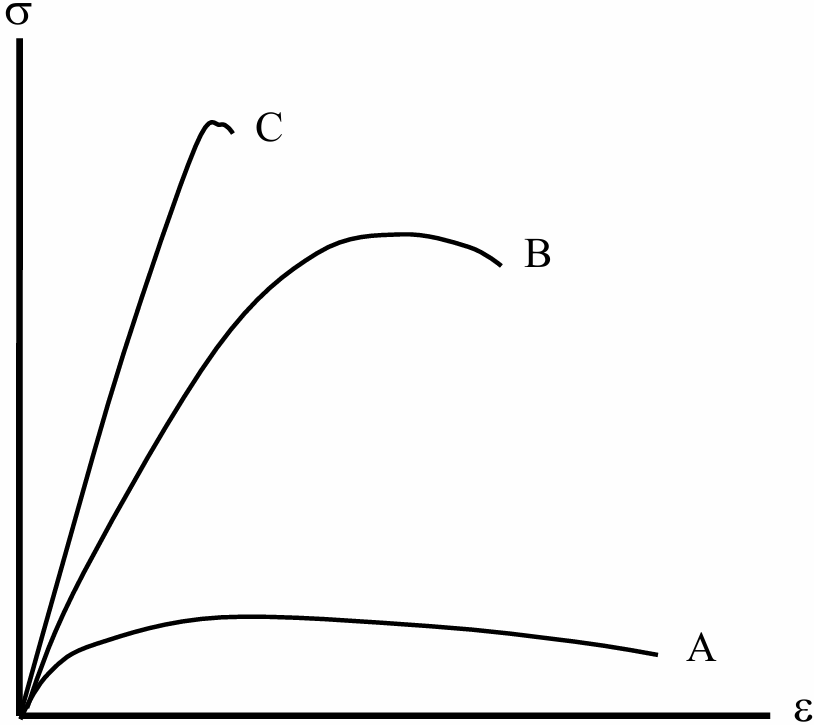
\includegraphics[width=0.5\textwidth]{stress_strain_curve.png}
\end{center}

\noindent \textbf{Figure:} Stress vs. Strain curves for samples A, B, and C.


\section*{Problem 4}

\noindent \textbf{Please determine true or false for the following statements (30 points, two points each):}

\begin{enumerate}
    \item[(a)] \textbf{True} \quad Ceramics usually have larger compressive strength than tensile strength.
    \item[(b)] \textbf{True} \quad The yield strength of polymers is typically affected by testing temperatures.
    \item[(c)] \textbf{False} \quad Elastic deformation is permanent while plastic deformation is temporary.
    \item[(d)] \textbf{False} \quad Plastic deformation is due to atomic bonding stretching.
    \item[(e)] \textbf{False} \quad Elastic deformation is related to dislocation motion.
    \item[(f)] \textbf{True} \quad Plastic deformation is related to dislocation motion.
    \item[(g)] \textbf{True} \quad FCC metals have 12 slip systems.
    \item[(h)] \textbf{False} \quad Slip results in a reversible elastic deformation.
    \item[(i)] \textbf{True} \quad The strength of a material is typically proportional to its hardness.
    \item[(j)] \textbf{True} \quad Creep refers to plastic deformation of a material at high temperature under constant load over an extended period of time.
    \item[(k)] \textbf{False} \quad Slip occurs most readily along crystal planes that are least densely populated.
    \item[(l)] \textbf{True} \quad Slip is impeded by solution hardening in which foreign atoms can serve as obstacles to dislocation motion.
    \item[(m)] \textbf{False} \quad One can use a fatigue tester to measure the impact energy of a material.
    \item[(n)] \textbf{False} \quad Ceramics typically have higher thermal conductivity.
    \item[(o)] \textbf{False} \quad A metal with BCC structure will not have ductile to brittle transition behavior.
\end{enumerate}

\section*{Problem 5}
\noindent \textbf{(Total 30 points)} A high-strength steel has a yield strength of \(1350 \, \text{MPa}\) and \(K_{IC}\) of \(100 \, \text{MPa} \sqrt{\text{m}}\). Assume that the geometric factor \(Y = 1\).

\begin{enumerate}
    \item[(a)] \textbf{Determine the length of a surface crack that will lead to catastrophic failure at an applied stress of \(3/4\) of the yield strength (10 points).}

    \begin{align*}
        K_{IC} &= Y \sigma \sqrt{\pi a} \\
        100 &= 1 \times \left(1350 \times \frac{3}{4}\right) \sqrt{\pi a} \\
        a &= 0.78 \, \text{mm}
    \end{align*}

    \item[(b)] \textbf{Determine the safe load stress if the maximum length of the internal cracks is \(5 \, \text{mm}\) (10 points).}

    \begin{align*}
        K_{IC} &= Y \sigma \sqrt{\pi a} \\
        100 &= 1 \times \sigma \sqrt{\pi \times 0.005} \\
        \sigma &= 898.94 \, \text{MPa}
    \end{align*}

    \item[(c)] \textbf{Determine the specimen thickness necessary to assure a valid \(K_{IC}\) measurement (10 points).}

    \begin{align*}
        \beta &\geq 2.5 \left(\frac{K_{IC}}{\sigma_Y}\right)^2 \\
        \beta &\geq 2.5 \left(\frac{100}{1350}\right)^2 \\
        \beta &\geq 3.43 \, \text{mm}
    \end{align*}
\end{enumerate}

\end{document}
